\section{Simulation}
\rhead{Simulation}

Der erste Schritt ist ein Modell zu erstellen.
Dazu wird der Golfstrom in drei Zonen aufgeteilt. Die jeweiligen Polarregionen und der Äquator werden je zu eine Zone. Diese Zonen erhalten dann je eine Box.
Im laufe des Seminars wurden zwei Modelle erstellt. Der erste Ansatz (siehe \ref{thermohalin:3b2f_title}) war sehr lehrreich hatte aber schlussendlich nichts mit dem realen Golfstrom gemeinsam. Der zweite Ansatz (siehe \ref{thermohalin:3b1f_title}) war erfolgreicher und der Golfstrom kann mit diesem Modell qualitativ simuliert werden.
In den folgenden zwei Kapiteln werden diese zwei Modelle vorgestellt und die jeweiligen Resultate diskutiert.

\subsection{Zwei-Fluss Modell( 1. Ansatz)}\label{thermohalin:3b2f_title}

In diesem Modell werden die Boxen jeweils durch Rohre verbunden wie im 2-Box Modell. Nun werden jedoch zwei Flüsse simuliert, die von den jeweiligen Dichtegradienten der unterschiedlichen Boxen abhängen. $q_1$ ist also nur vom Dichteunterschied zwischen Box $1$ und Box $2$ abhängig. Dementsprechend hängt auch $q_2$ nur vom Dichteunterschied der Boxen $2$ und $3$ ab.
Der Vorteil der Aufteilung der Flüsse ist, dass wir sie entkoppeln können und sie nicht von der jeweiligen dritten Box abhängig sind.
Eine Darstellung des Modelles ist in Abbildung 9.4 zu finden.

\begin{figure}
	\centering
	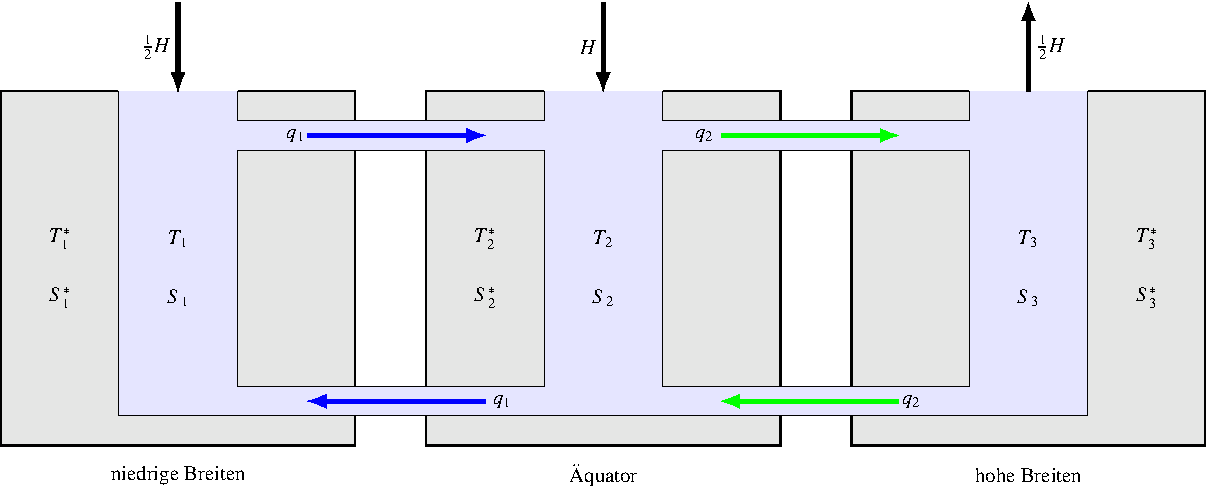
\includegraphics[width=14cm]{thermohalin/tikz/3b2f.pdf}
	\caption{Zwei-Fluss Modell des THC}
		\label{thermohalin:3b2f}
\end{figure}

So lassen sich nun für jede Box die zugehörigen Salinitäts- und Temperaturgleichungen aufstellen. So ist auch ersichtlich, dass Box $1$ und $3$ jeweils einen Fluss in der Gleichung haben. Im Gegensatz dazu hat Box $2$ jedoch zwei Flüsse in der Gleichung. Das liegt daran, dass wie aus der Abbildung ersichtlich, die mittlere Box von beiden Strömen durchflossen wird.


\begin{equation}\label{thermohalin:diffgl_3b2f}
\begin{aligned}
\frac{dT_1}{dt} &= c(T_1^*-T_1)&+|q_1|(T_2-T_1)\phantom{+|q_2|(T_3-T_2)}
\\
\frac{dT_2}{dt} &= c(T_2^*-T_2)&+|q_1|(T_1-T_2)+|q_2|(T_3-T_2)
\\
\frac{dT_3}{dt} &= c(T_3^*-T_3)&+ \phantom{+|q_1|(T_1-T_2)}|q_2|(T_2-T_3)
\end{aligned}
\end{equation}
\begin{equation}
\begin{aligned}
\frac{dS_1}{dt} &= -\frac{H}{2} &+ d(S_1^*-S_1)&+|q_1|(S_2-S_1)\phantom{+|q_2|(S_3-S_2)}
\\
\frac{dS_2}{dt} &= \phantom{-}H &+ d(S_2^*-S_2)&+|q_1|(S_1-S_2)+|q_2|(S_3-S_2)	
\\
\frac{dS_3}{dt} &= -\frac{H}{2} &+d(S_3^*-S_3)&+ \phantom{+|q_1|(S_1-S_2)}|q_2|(S_2-S_3)
\end{aligned}
\end{equation}	

Die Flussgleichungen entstehen wie beim Zwei-Box Modell aus dem Dichteunterscheid zwischen den jeweiligen Boxen. 
Die jeweiligen $q$ sind also 
\begin{equation}
\begin{aligned}
	q_1 &= k\frac{\varrho_1-\varrho_2}{\varrho_0}
	\\
	q_2 &= k\frac{\varrho_2-\varrho_3}{\varrho_0}
\end{aligned}
\end{equation}.

Weiter kann dann die Formel für die Dichte eingesetzt werden.

\begin{equation}
\begin{aligned}
q_1 &= k\frac{\varrho_0[1-\alpha(T_1-T_0)+\beta(S_1-S_0)]-\varrho_0[1-\alpha(T_2-T_0)+\beta(S_2-S_0)]}{\varrho_0}
\\
q_2 &= k\frac{\varrho_0[1-\alpha(T_2-T_0)+\beta(S_2-S_0)]-\varrho_0[1-\alpha(T_3-T_0)+\beta(S_3-S_0)]}{\varrho_0}
\end{aligned}
\end{equation}

$\varrho_0, T_0$ und $S_0$ lassen sich kürzen, sodass am Schluss folgende Flussgleichungen entstehen.

\begin{equation}
\begin{aligned}
 q_1 &= k[\alpha(T_2-T_1)-\beta(S_2-S_1)] 
 \\
 q_2 &= k[\alpha(T_3-T_2)-\beta(S_3-S_2)]
\end{aligned}
\end{equation}

Da die Flüsse nur von den Differenzen der jeweiligen Boxen abhängig sind, kann man sie auch so schreiben:

\begin{equation}
\begin{aligned}
q_1 &= k[\alpha(\Delta T_{q1})-\beta(\Delta S_{q1})] 
\\
q_2 &= k[\alpha(\Delta T_{q2})-\beta(\Delta S_{q2})]
\end{aligned}
\end{equation}

\subsubsection{Matlab-Code der Simulation}

Ziel ist es, die oben aufgestellten Differentialgleichungen ( \ref{thermohalin:diffgl_3b2f}) mittels Matlab zu lösen. Dies wird mit dem Differentialgleichungslöser \texttt{ode45} aus der Matlab Funktionenbibliothek erreicht.
Dazu müssen wir der Funktion einen Zustandsvektor, einen Zeitvektor und die Konstanten der jeweiligen Reservoirtemperaturen und Reservoirsalinitäten übergeben.
\begin{equation*}
y_0 = \begin{pmatrix}T_{1} \\ T_{2} \\ T_{3} \\ S_{1} \\ S_{2} \\ S_{3}\end{pmatrix}, \quad
t_{span} = \begin{pmatrix}t_0 \\ t_{end} \end{pmatrix}, \quad
const = \begin{pmatrix}T_{1}^{*} \\ T_{2}^{*} \\ T_{3}^{*} \\ S_{1}^{*} \\ S_{2}^{*} \\ S_{3}^{*}\end{pmatrix}
\end{equation*}




\lstinputlisting[style=Matlab]{thermohalin/listings/input.m}\label{thermohalin:listing:input}
Diese werden dem Differentialgleichungslöser übergeben.
\lstinputlisting[style=Matlab]{thermohalin/listings/listing-ode45.m}\label{thermohalin:listing:uebergabe}

Daraufhin wird im File \texttt{odefun-3Box.m} das Gleichungssystem schrittweise gelöst und die Resultate zurückgegeben. Gleichzeitig wird der Zustandsvektor mit $0$ initialisiert und die Naturkonstanten zur Flussberechnung definiert.

\lstinputlisting[style=Matlab]{thermohalin/listings/listing-solve.m}\label{thermohalin:listing:solve}

Die Rückgabewerte werden in einem Array gespeichert und dann geplottet. Um den Text nicht in die Länge zu ziehen wird hier nur der Code zur Erstellung des Temperaturplots dargestellt. Die Salinität folgt dem gleichen Schema.
Da die Flüsse innerhalb der ode45-Funktion berechnet wurden, muss dies nachträglich noch einmal gemacht werden, um die Werte nachher plotten zu können. Dazu müssen die jeweiligen Werte aus dem Lösungsvektor extrahiert und die Flüsse wiederholt berechnet werden.
\lstinputlisting[style=Matlab]{thermohalin/listings/listing-plot.m}\label{thermohalin:listing:plot}

Die so entstehenden Figuren werden im folgenden Kapitel ausgewertet und diskutiert. 

\subsubsection{Resultate}


Soweit sieht alles vielversprechend aus und die ersten Durchläufe ergaben auch brauchbare Resultate. Wenn nun jedoch mit den Temperaturen und Salinitäten der Reservoire ( $S_1^*, T_1^*,...$) verändert werden, treten plötzlich unmögliche Phänomene auf.
Einer der beiden Flüsse wird negativ und ändert seine Richtung. Das resultiert in zwei gegenläufigen Strömen welche in keiner Weise mit dem Golfstrom übereinstimmen. Das führt dazu, dass am Äquator eine Absinkstelle entsteht. In der Realität ist klar zu erkennen, dass Absink- und Aufsteigstellen jeweils nur an den Polen vorhanden sind. 
Ein Plot der Simulationsresultate findet sich in Abbildung \ref{thermohalin:simulationsresultate}.

\begin{figure}
	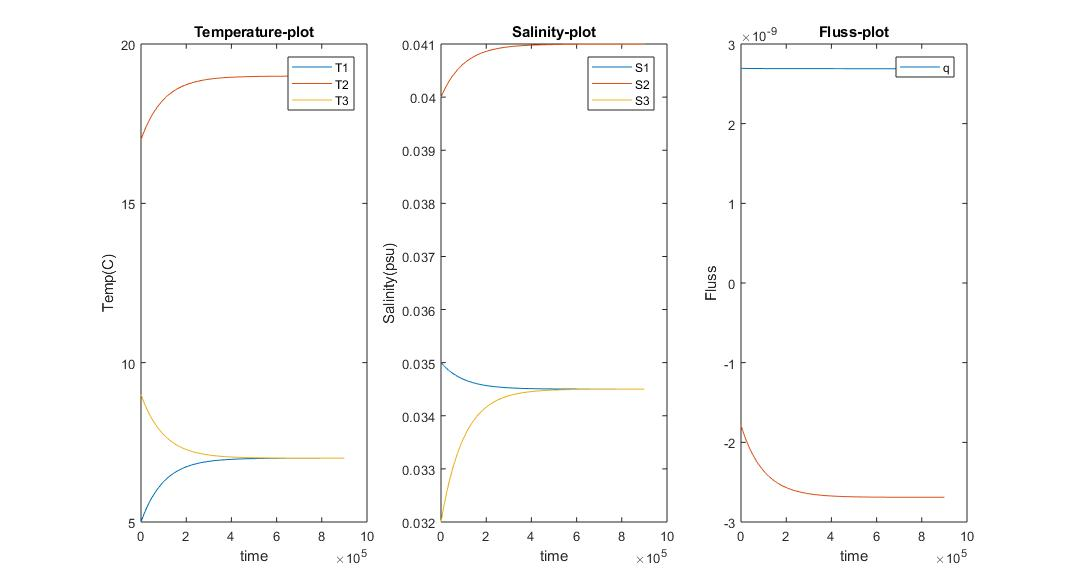
\includegraphics[width=14cm]{thermohalin/Code/graphs/result-3b2f-script.jpg}
	\centering
	\caption{Simulationsresultate}
	\label{thermohalin:simulationsresultate}
\end{figure}

Durch die Entkoppelung der zwei Flüsse, war es möglich, dass ein Fluss seine Richtung ändert.
Die Simulation hat zwar funktioniert, nur ist das Modell fehlerhaft. Wir müssen also unsere Darstellung des Modells anpassen. In der mittleren Box muss eine Absinkstelle eingefügt werden, damit das Modell mit der Simulation übereinstimmt. Das Resultat der Anpassung ist in Abbildung \ref{thermohalin:3b2f-inverted} zu sehen.

\begin{figure}
	\centering
	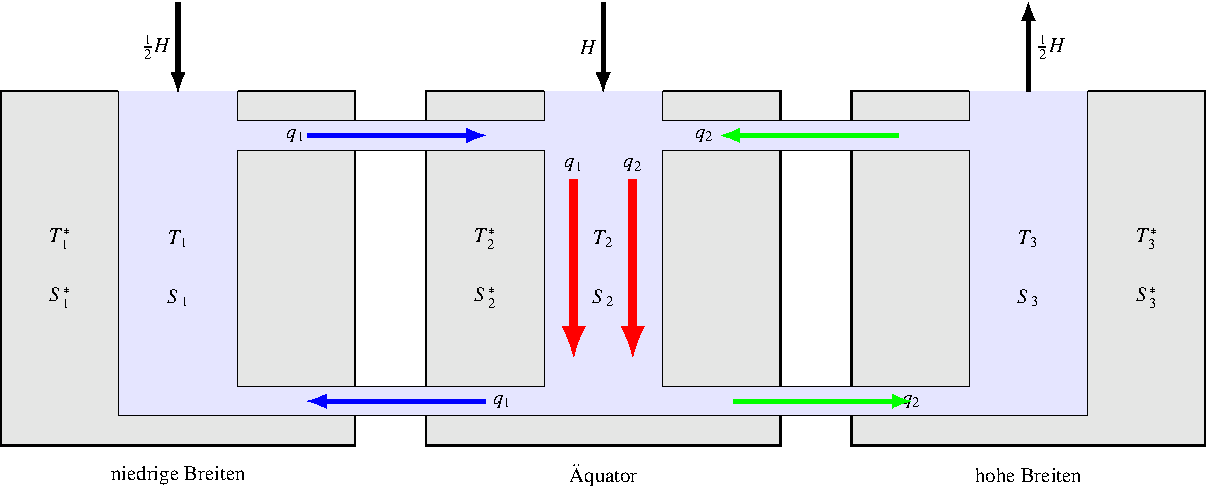
\includegraphics[width=14cm]{thermohalin/tikz/3b2f-inverted.pdf}
	\caption{Angepasstes Zwei-Fluss Modell}
	\label{thermohalin:3b2f-inverted}
\end{figure}

Nun lässt sich die neu entstandene Absinkstelle auch sofort erkennen. 
Mit diesem Modell lässt sich der Golfstrom also nicht erfolgreich simulieren. 

\subsection{Ein-Fluss Modell (2. Ansatz)}\label{thermohalin:3b1f_title}

Dieses Modell ist der verbesserte Nachfolger des Zwei-Fluss Modelles.
Es stammt aus einer Aufgabe von \texttt{\em Mathematics and Climate} \cite{skript:kaperengler}.

Um zu verhindern, dass in der mittleren Box eine zusätzliche Absinkzone entsteht, muss dieser Weg versperrt werden. Das erreicht man am einfachsten, wenn der Tiefenstrom von der Äquatorbox getrennt wird. Die Äquatorzone ist nur via Oberflächenströmungen mit den anderen Boxen verbunden und die Tiefenströmung verbindet die Polzonen.


\begin{figure}
	\centering
	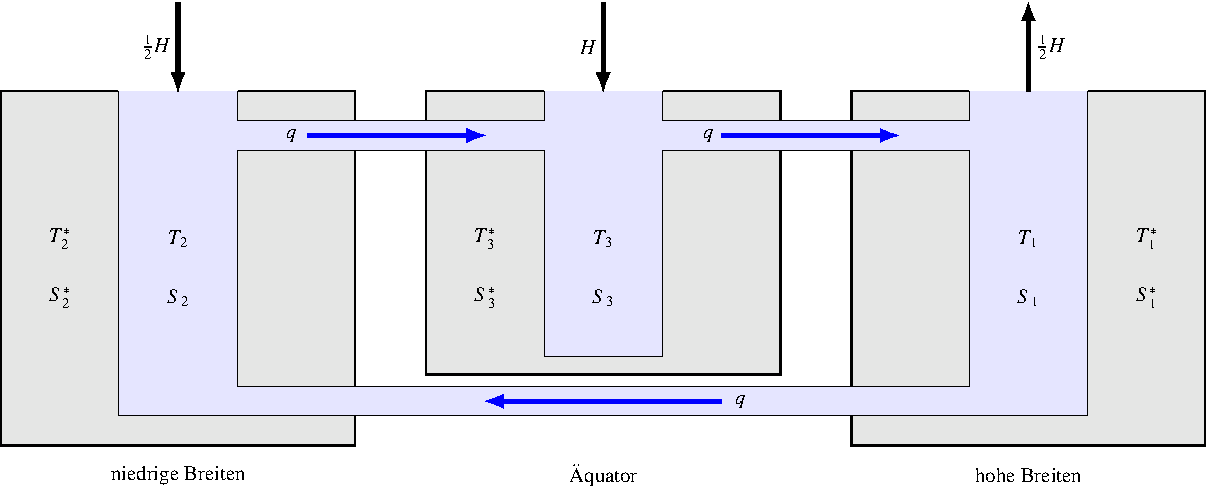
\includegraphics[width=14cm]{thermohalin/tikz/3b1f.pdf}
	\caption{Ein-Fluss Modell des THC}
	\label{thermohalin:3b1f}
\end{figure}

Wie im vorherigen Modell benötigen wir drei Gleichungen für Temperatur- und Salinitätsänderung der jeweiligen Boxen.
Jedoch gibt es nur noch einen Fluss welchen die Boxen verbindet. Das stimmt auch viel besser mit der Realität überein. Folgend ist die Gleichung für Box Nr. 1 dargestellt, um die Zusammenhänge zu erläutern:

\begin{equation}
\frac{dT_1}{dt} = c(T_p-T_1)+ \begin{cases} q(T_3-T_1)  \quad q>0 \\ |q|(T_2-T_1)  \quad q<0 \end{cases}
\end{equation}

Der erste Term beschreibt wie bisher den Temperaturaustausch zwischen Box und Reservoir. Der zweite Term ist jedoch anders, da der Fluss je nach Flussrichtung von anderen Boxen getrieben wird. Die Differenz muss jeweils zwischen der Quellbox und der betrachteten Box berechnet werden, da der Energie- und Salztransport jeweils nur vom Unterschied abhängt.
Wenn der Fluss positiv ist, also $q>0$, dann wird für die Berechnung Box 3 und die aktuelle Box verwendet, da die dritte Box die Quellbox darstellt. Wenn der Fluss nun negativ wird, ist die Quellbox jedoch Box 2 also muss hier die Differenz zwischen der zweiten und der dritten Box berechnet werden. Um die Simulation zu erleichtern, wird im Falle eines negativen Flusses mit dem Absolutbetrag gerechnet. Damit die Resultate trotzdem stimmen werden  bei der Differenzbildung jeweils die Terme vertauscht damit die Richtung trotzdem korrekt ist. 

Der Fluss wird ebenfalls anders berechnet, er ist nur vom Dichteunterschied zwischen den jeweiligen Polen abhängig \cite{skript:kaperengler}.
Wir können also wieder schreiben

\begin{equation}
q = k\frac{\varrho_1-\varrho_2}{\varrho_0}
\end{equation}

woraus folgt

\begin{equation}
q= k\frac{\varrho_0[1-\alpha(T_1-T_0)+\beta(S_1-S_0)]-\varrho_0[1-\alpha(T_2-T_0)+\beta(S_2-S_0)]}{\varrho_0}
\end{equation}

Das lässt sich wieder kürzen, woraus sich folgende Gleichung für den Fluss ergibt:

\begin{equation}
q = k[\alpha(T_2-T_1)-\beta(S_2-S_1)] 
\end{equation}

Die Gleichungen für die anderen Boxen lassen sich nach dem gleichen Schema erstellen. Nur müssen jeweils entsprechend der Flussrichtung andere Quellboxen verwendet werden. Das gesamte Gleichungssystem hat dann folgende Form

\begin{equation}
\begin{aligned}
\frac{dT_1}{dt} &= c(T_p-T_1)&+ \begin{cases} q(T_3-T_1) & \quad q>0 \\ |q|(T_2-T_1) & \quad q<0 \end{cases}
\\
\frac{dT_2}{dt} &= c(T_p-T_2)&+\begin{cases} q(T_1-T_2) & \quad q>0 \\ |q|(T_3-T_2) & \quad q<0 \end{cases}
\\
\frac{dT_3}{dt} &= c(T_e-T_3)&+\begin{cases} q(T_2-T_3) & \quad q>0 \\ |q|(T_1-T_3) & \quad q<0 \end{cases}
\end{aligned}
\end{equation}
\begin{equation}
\begin{aligned}
\frac{dS_1}{dt} &= -H/2 &+ d(S_p-S_1)&+\begin{cases} q(S_3-S_1) & \quad q>0 \\ |q|(S_2-S_1) & \quad q<0 \end{cases}
\\
\frac{dS_2}{dt} &= \phantom{-}H &+ d(S_p-S_2)&+\begin{cases} q(S_1-S_2) & \quad q>0 \\ |q|(S_3-S_2) & \quad q<0 \end{cases}	
\\
\frac{dS_3}{dt} &= -H/2 &+d(S_e-S_3)&+\begin{cases} q(S_2-S_3) & \quad q>0 \\ |q|(S_1-S_3) & \quad q<0 \end{cases}
\end{aligned}
\end{equation}

\begin{equation}
q = k[\alpha\Delta T-\beta\Delta S] 
\end{equation}.



Aufgrund diese Gleichungen kann dann der neue Matlabcode geschrieben werden, welcher im nächsten Abschnitt erklärt wird.


\subsubsection{Matlab-code}

Die Übergabe der Startwerte und Konstanten, der Aufruf des Differentialgleichungslösers und das Plotten der Resultate sind gleich geblieben und werden deshalb nicht noch einmal gezeigt ( siehe  \ref{thermohalin:listing:input}). Die Änderungen befinden sich in der Funktion selber. Je nachdem ob der Fluss positiv oder negativ ist muss ein anderer Fall der Gleichung berechnet werden. Dies wird mit einem \texttt{if}-Statement erreicht, welches in jedem Durchgang neu ausgewertet wird. 

\lstinputlisting[style=Matlab]{thermohalin/listings/listing-3b1f-solve.m}


\subsubsection{Resultate} 

Nach mehrfacher Simulation scheint es so, dass dieses Modell tatsächlich funktioniert. Für Werte, welche realen Werten entsprechen, reagiert die Simulation wie der richtige Golfstrom. Der Golfstrom fliesst vom Süd- zum Nordpol, sinkt dort ab und fliesst am Meeresgrund wieder bis zum Südpol, wo er aufsteigt und so den Kreislauf schliesst. Ein Plot der Resultate ist in Abbildung \ref{thermohalin:3b1f-skript} dargestellt.

Wie ersichtlich wird, bleiben die Temperaturen ungefähr konstant. Dies liegt daran, dass die Temperaturstartwerte schon den Reservoirwerten angepasst wurden, was bedeutet dass diese Anpassung schon geschehen ist. Beim Salinitätsplot ist jedoch klar der Effekt des virtuellen Salzflusses zu sehen, welcher dazu führt, dass die Salinität in der Äquatorregion leicht steigt und in Polnähe dementsprechend abnimmt. Das Resultat stimmt jedoch und der Golfstrom fliesst in die uns bekannte Richtung.

\begin{figure}
	\centering
	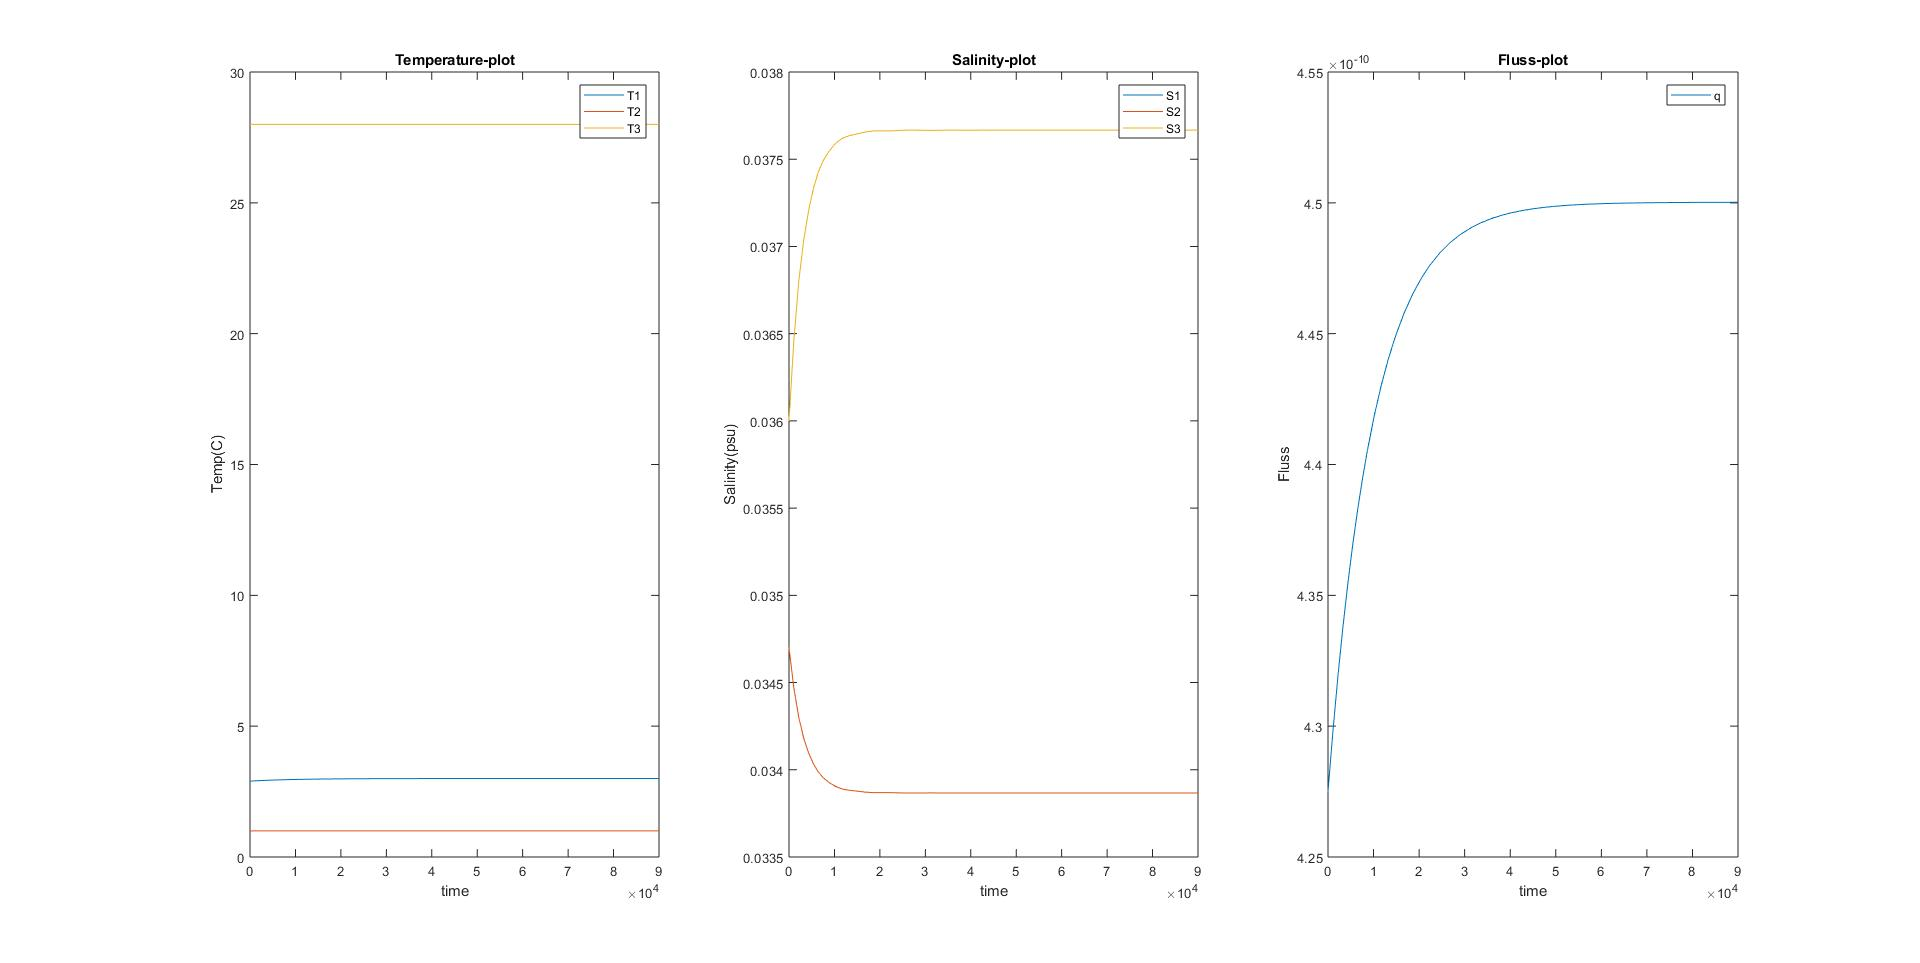
\includegraphics[width=14cm]{thermohalin/Code/graphs/3b1f-skript.jpg}
	\caption{Resultat der Ein-Fluss Simulation ohne Klimawandel}
	\label{thermohalin:3b1f-skript}
\end{figure}

Spannend wird es nun, wenn die Reservoirvariablen so angepasst werden, dass sie eine Klimaerwärmung und deren Folgen darstellen. Wie bereits in Abschnitt \ref{thermohalin:EinflussKlimawandel} erläutert, muss dazu die Salinität am Nordpol und die Temperatur am Äquator erhöht werden. Dies sollte dazu führen, dass der Golfstrom schwächer wird, anhält oder gar seine Richtung ändert. 
Der Eingabevektor, welcher die Temperaturen und Salinitäten der Reservoire enthält wird also angepasst.
Die Werte von $S_1^*$ ( Salinität Nordpol) und $T_3^*$ (Temperatur Äquator) werden also erhöht.

\begin{equation*}
const = \begin{pmatrix}T_{1}^{*} \\ T_{2}^{*} \\ T_{3}^{*} \\ S_{1}^{*} \\ S_{2}^{*} \\ S_{3}^{*}\end{pmatrix}
\end{equation*}



Bei einer kleinen Veränderung wird der Strom nur schwächer, je grösser die Abweichungen jedoch sind desto stärker wird der Effekt.
Bis sich die Richtung des Stromes ändert.
Das Resultat entspricht also den Erwartungen. 

\begin{figure}
	\centering
	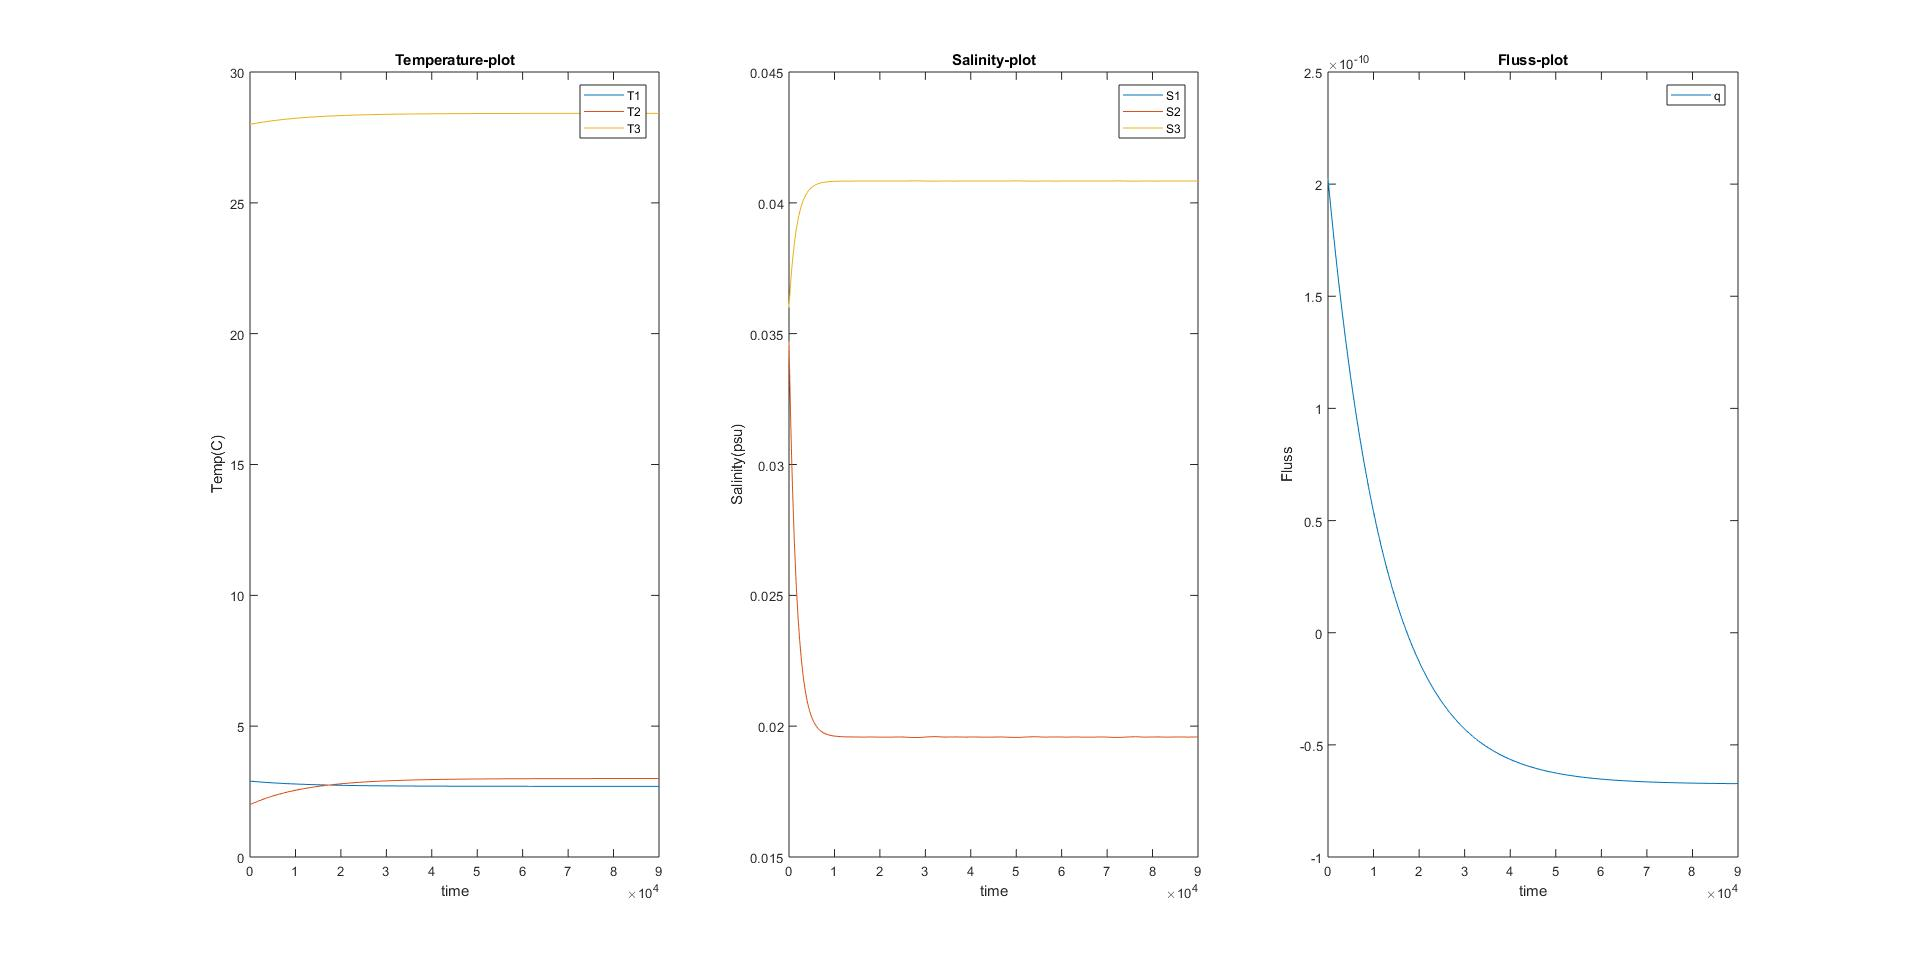
\includegraphics[width=14cm]{thermohalin/Code/graphs/3b1f-skript-klimawandel.jpg}
	\caption{Resultat der Ein-Fluss Simulation mit Klimawandel}
	\label{thermohalin:3b1f-skript-klimawandel}
\end{figure}

Wenn das nun mit dem Paper von Liu Wei \cite{thermohalin:liuwei} vergleichen, kommen wir auf vergleichbare Resultate.


